\section{Materiales y métodos}

Se ha llevado a cabo un estudio fenotípico sobre la población afectada por el fenómeno de Raynaud. Se pretende averiguar la influencia de los diferentes genes asociados a la enfermedad y su grado de importancia en el desarrollo de la misma.

Para llevar acabo la siguiente metodología hemos será necesario descargar la última versión de R, que, hasta la fecha de este proyecto es la 4.2.1 . Así como será necesario instalar todas las librerías indicadas en el repositorio de gitHub.

\begin{minipage}{\linewidth}
	\vspace{15pt}
	\makebox[\linewidth]{
		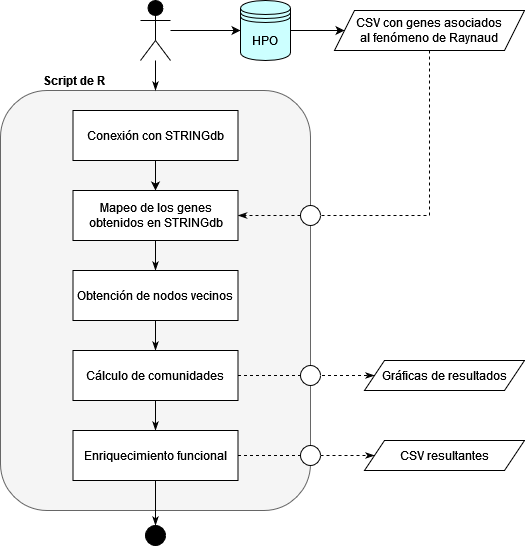
\includegraphics[width=0.6\textwidth]{figures/Workflow_genes.png}
	}
	\vspace{3pt}
	\captionof{figure}{Flujo de trabajo}
	\label{fig:workflow}
\end{minipage}

\subsection{Obtención de la red}

STRINGdb es una base de datos open-source que busca integrar todas las relaciones conocidas entre proteínas, así como sus interacciones físicas o funcionales. Esta herramienta también nos permite visualizar las redes que forman un conjunto de proteínas. Para la obtención automática de los datos es necesario utilizar la API de STRINGdb con R. Al tratarse de un estudio sobre una enfermedad que afecta a humanos, es necesario descargar de 'string' todas las proteínas, interacciones y peso de el enlace; del genoma humano al completo. El ID taxonómico con el que realizar la búsqueda es el \textbf{9606}. Como ya se ha comentado en el apartado \ref{genes_asociados} y como podemos ver en \ref{fig:workflow} es necesario descargar de HPO el nombre de los genes asociados, su rentrez\_ID (que será útil para el mapeo de nuestros genes en el genoma) y el identificador del gen de la base de datos de OMIM; Todos estos datos relacionados con el fenómeno de Raynaud.

\subsection{Cálculo de comunidades}
\subsection{Enriquecimiento funcional}
